% !TeX spellcheck = en_US
 
\chapter{Tools} %Das ist nur ein Arbeitstitel
\section{Template}
\subsection{Toolname}
\label{Toolname} % to refernce in the document
Introduction Text with all infos about contributors and installation Process
\subsubsection{Appearance}%Only for Visual tools
Description of the tool front-end with a Screen shot of the homepage/Dashboard
\subsubsection{Performance}
Quick analysis of the Performance (CPU/RAM usage during the test)
\subsubsection{Interoperability}
Which tools are listed to work with the tool/Which tools are test to work with the tool
\subsubsection{Conclusion}
A Quick Pro/Con of the tool and in which environment its best to use
\section{Installed Tools}%Arbeitstitel
\subsection{Searchlight (Icinga)}
\label{searchlight}
As in the Section Icinga \ref{Icinga} described, we were not able to find a pure installation of Icinga for a cluster so we tried to install Searchlight as a backup plan.
Searchlight is a tool from the AppsCode Inc. (\url{https://appscode.com/},18.12.2017) which is a company located in San Leandro Californian. 
Searchlight is as many other monitoring tools written in the Programming language of Go.
\\
When first trying this over the yaml File we resived errors over the Kubernetes Cluster. There it says the tools is not able to bind the Port 8443. We could not figure out wich Apllication is using the port but as we tried to install the app on a fresh cluster VM it turns out the yaml deployment is working fine.
\subsubsection{Appearance}
%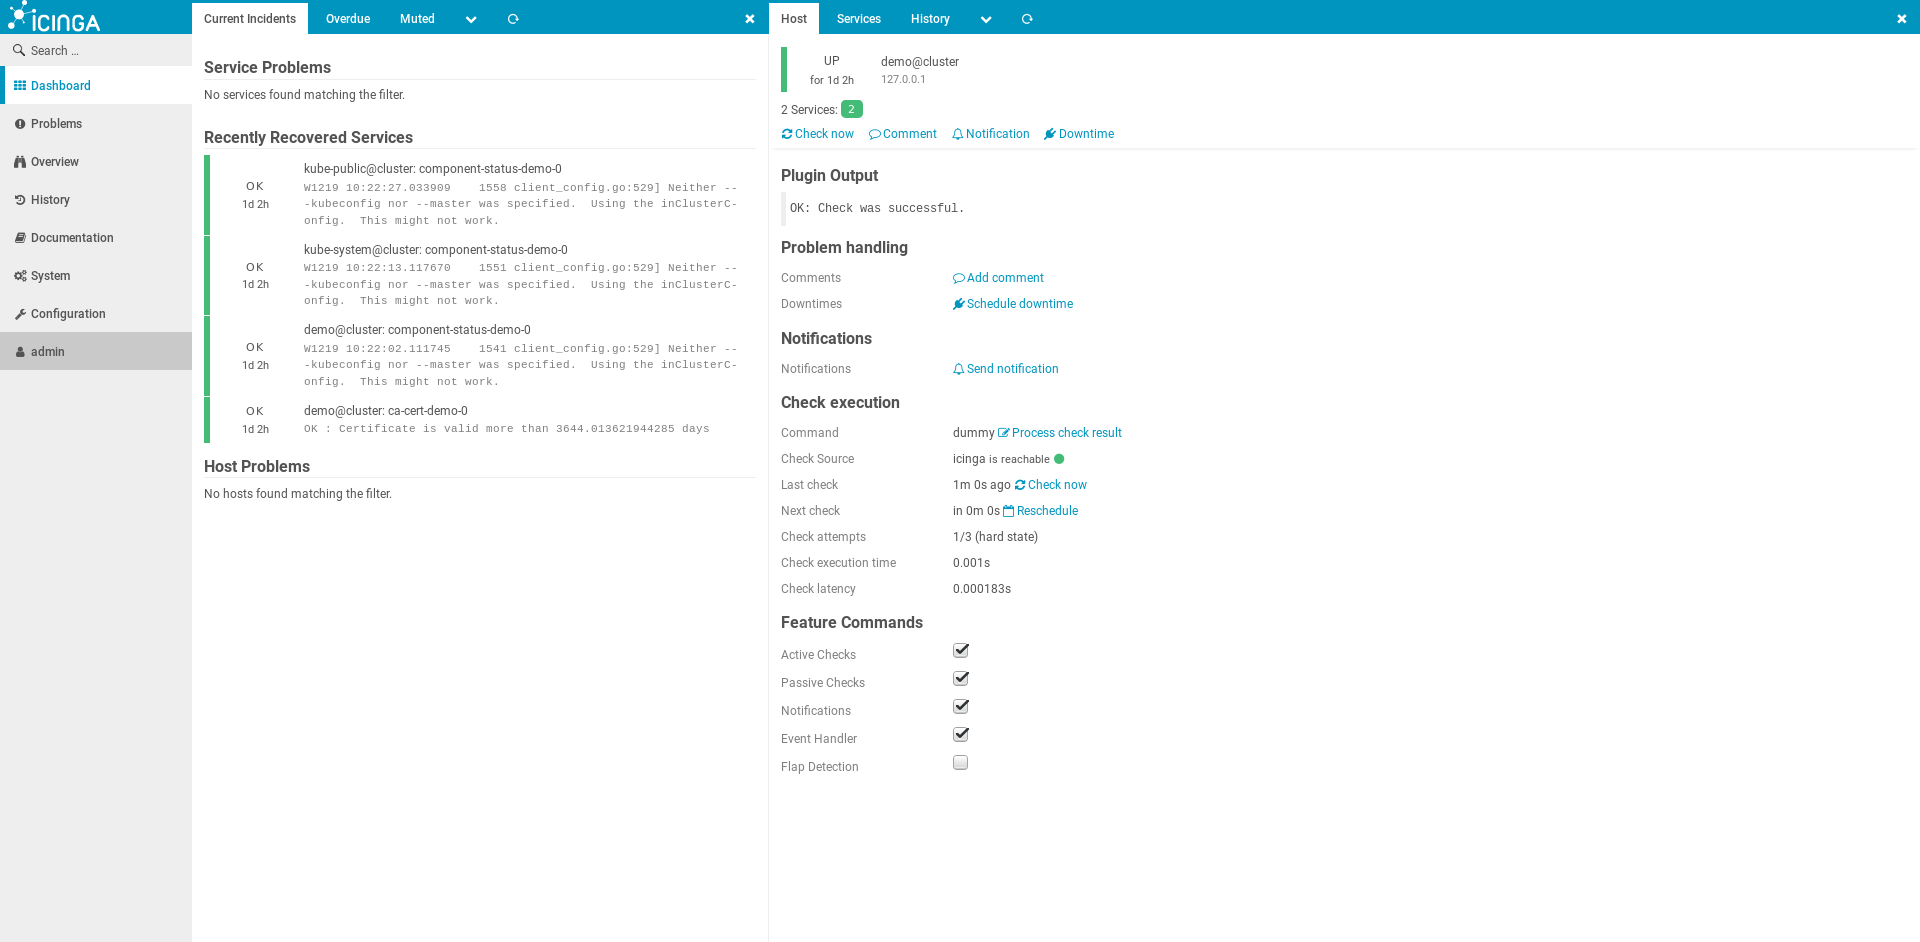
\includegraphics[width=1\linewidth]{Bilder/Searchlight_Icinga}\\
Icinga/Searchlight comes in a  discreet blue/withe coloring. On the Dashboard which represents the homepage of the application an overview of the implemented alerts is shown. The alerts will be Colored with Green/Yellow/Red for OK/Warning/Error, so its easy to see appearing problems. The rest of the option as History and Configurations is located at the sidebar. 
\subsubsection{Performance}
In our VM deployment the applications has allocated 160MB of RAM under Load. The Application it self is Running very smooth even on low Power Systems. As we deployed some alerts we noticed that it took about 30 seconds to validate the alert and get a first status from the system. After that pending status run Smoothly and even checks on a 30 seconds bases were no Problem for the System.
\subsubsection{Interoperability}
On the Github Page (\url{https://github.com/appscode/searchlight},20.12.2017) of the Program the developer claims to be able to send Notification over Email, SMS and Chat.
In the Guide there is no explicit explanation what is meant by the term Chat but the tool is cable to send Notifications to Slack(\url{https://slack.com},03.01.2018) and Hipchat. Notification over Email can be without any third party Software send over SMTP. To send SMS a Service like Twilio(\url{https://www.twilio.com/},20.12.2017) is needed.
On the page there is no advise that the tool is capable of interaction over an over interface then Notification. 
\subsubsection{Conclusion}
Searchlight is a light weighted  port of the famous monitoring tool Icinga. It runs well and has all Basic needed Features. On a deeper Look the Software revaled its weekneses. There are no advanced Possibilities to connect Searchlight with over Monitoring tool. Also there is no Graphical user interface for creating alerts, which makes it very difficult to set it up. As the tool is manly only developed and updated by 2 two people the support for new Version of Icinga and Kubernetes is limited. The fact that the company appcode has no direct correlation with Icinga is a nother counter-argument to the tool. In a nutshell the tool is good for small Kubernetes clusters that want to monitor only a few Basic metrics and have low resources. 

\subsection{Prometeus}
\label{Toolname} % to refernce in the document
The tool Prometeus is a open source Project and is hosted by the Cloud Native Computing Foundation. The project was originally built at Soundcloud. The tool can be installed on an os or on cluster like Kubernetes. Because the project is community driven, there is no official repository for Kubernetes, but with a little research we managed to find this repository (https://github.com/kayrus/prometheus-kubernetes,10.01.2018) which provides different deployments for Kubernetes.

We managed to install Prometeus so that we were able to get metrics from the Api-server and can expose them over a restful interface. Over this interface it was possible to connect Prometeus to a application outside or inside the cluster like Grafana which is recommended for Prometeus. We were not able to install the Promteus own alertmanger on the cluster. Also we were not able to get metrics from the cluster-nodes because the Prometeusversion is not cable of requesting over https. 
\subsubsection{Appearance}%Only for Visual tools
Prometeus provides a web ui for user to see the collected data. It is designed in a very light wighted black an with combination with some blue ascents and only shows the necessary things. The interface has no function to save the set of graphs that is selected and no option to login to keep the data save or to divide the data by some user groups.   
\subsubsection{Performance}
The tool is very quickly booted and shows no Performance problems on the interface. A look on the stats shows that Prometeus is not very CPU dependent but takes up to 2GB of RAM. These high numbers of RAM is allocated over a time from about 24h. 
\subsubsection{Interoperability}
It's highly recommended that Prometeus is used with a Graphing and alerting tool because its just a collector and time series database with a query engine. In our Deployment Graphana is used, which is also recommended by the Prometeus web page (\url{https://prometheus.io/},12.01.2018). Exploiting Prometheus to any other tool is also possible as Prometeus provides the metrics that are collected in plain text
\subsubsection{Conclusion}
Prometeus is very good as a Collector for large Kubernetes Clusters with hundreds or thousands of nodes. What makes it so good is the With-Box monitoring approach, which provides way more metrics than a black-box monitoring. These fact can be used to detect problems in the system earlier and in much more detail so that the downtime can be reduced. On the over side Prometeus is not good for presenting this data and to throw alerts in case of failure.

\subsection{Zabbix}
\label{Toolname} % to refernce in the document
% \url{https://dl.acm.org/citation.cfm?id=1883485} Linux Journal
The tool Zabbix is an open-source tool and is developed by Zabbix LLC (Limited Liability Company) since 2005 (\url{https://www.zabbix.com},15.01.2018). Zabbix provides a all in one Solution with includes a Collector, Database, Visualization tool and a alert manager. Moreover there is a repo from monitoringartist (\url{https://github.com/monitoringartist/kubernetes-zabbix},15.01.2018) that provides a yaml which maps Zabbix client and server on a cluster structure.  
\subsubsection{Appearance}%Only for Visual tools
Zabbix come with a withe and blue web interface with some Red accents. It implements a tab system with subtabs to navigate through the interface. The naming itself is not as explaining as it could be.  
\subsubsection{Performance}
The general Performance of Zabbix is very good. The three parts in hole take up to 1GB of ram of the System and about 0.5 \% of the Processor load.
\subsubsection{Interoperability}
Which tools are listed to work with the tool/Which tools are test to work with the tool
\subsubsection{Conclusion}
A Quick Pro/Con of the tool and in which environment its best to use

\section{Failed Tools}%Ebenfalls nur ein arbeitstitel
In the Process of Developing and Evaluating the APM we Discoverd a bunch of Tools that we were not able to install even that they clamed to be optimized to work on Kubernetes .
In this Paragraph all the tools we wanted to include in our Report but doesn't are mentioned with a quick description of the Failure.
\subsection{Graphite}
Graphite is mainly for storing and Graphing data and metrics, but brings also tools that are able to collect these Metrics from the system. By the Developer it self there is no Kubernetes installation Provide but there are diverse approaches by third party members to make it runnable on a Cluster. We have tested the Repository from nanit\\(\url{ https://github.com/nanit/kubernetes-graphite-cluster},11.12.2017) to get Graphite running with StatsD (\url{https://github.com/etsy/statsd.git},11.12.2017) as a metric collection tool. The Repo doesn't provide a yaml file by it self to install all the tools. The instruction leads the user to export some Variables needed for the installation. After that a deploy command is provided that pulls the docker repo and than installs it with kubectl on the Cluster. As we tried to execute this command a fail was thrown, The Node Replicas were empty, so no further commands are executable. As we were not able to install the tool on multiple Kubernetes Clusters, we installed the tool as on the Webside advertised on a Ubuntu System directly. With this installation of Graphit a time-series Data,an Monitoring and an Alerting tool is included. On the test System the Monitoring System gave values that differs from the Linux intern monitoring in values like Cpu usage or RAM. As a Solution to all this Difficulties we decided to not perform further test on the tool.

\subsection{Icinga}
\label{Icinga}
Icinga is as ELK-Stack not a Monitoring tool. Its made for logging defined Request. The Adminestrator can decide which system to monitor an in what interval the data is pulled.
Icinga it self only provides 3 system states instead of exact values. The states are OK/Warning and Error. The user decieds at which point they are triggered.\\
As we tried to install Icinga as we found out that there was no direct support from Incinga for Kubernetes. As our Study only describes the actual state without trying to add somthing we decidet not to try an compile Icinga into Kuberntes on oure own. Later we found out there is a third party Software called searchlight \ref{searchlight}. Its provided by appscode on github.
 